\documentclass[12pt]{article}
\title{\textbf{DataPrivacy—hw1}}
\author{\textbf{Terence Wang}}% 作者
\date{\textbf{2023/11/05}}% 日期
\usepackage[colorlinks=true]{hyperref}  % 为文档中的章节引用自动添加链接
\usepackage{color}% 调用颜色宏包
% \setlength{\parindent}{4em} %设置首行缩进
\usepackage{fancyhdr} %页眉、页脚
\usepackage{enumitem}
\usepackage{sectsty}
\pagestyle{fancy}
\lhead{}
\chead{}
\rhead{\bfseries DataPrivacy—hw} %页眉内容
\lfoot{\bfseries WANGYU} %页脚内容
\cfoot{\bfseries PB21030814} %页脚内容
\rfoot{\thepage} %在页脚处给出页码
\renewcommand{\headrulewidth}{0.4pt}
\renewcommand{\footrulewidth}{0.4pt}
\usepackage{algorithm}
\usepackage{algorithmic}
\usepackage{amsmath, amsfonts}
\usepackage{graphicx} %插入图片
\usepackage{caption}
\usepackage{hyperref}
\usepackage{colortbl}



\begin{document}
\maketitle
\tableofcontents
\newpage

\section{Q1}
\subsection{a}
The quasi-identifier attributes: \textbf{Zip Code}\quad \textbf{Age}\quad \textbf{Salary}\quad \textbf{Nationality}
\subsection{b}
After cell-level generalization:
\newline
\begin{tabular}{|l|l|l|l|l|l|}
    \hline
    Sequence & Zip Code & Age     & Salary    & Nationality & Condition       \\
    \hline
    1        & 130**    & [21,40] & [13k,22k] & *           & Heart Disease   \\
    \hline
    2        & 130**    & [21,40] & [23k,25k] & *           & Heart Disease   \\
    \hline
    3        & 130**    & [21,40] & [13k,22k] & Japanese    & Viral Infection \\
    \hline
    4        & 130**    & [21,40] & [13k,22k] & *           & Viral Infection \\
    \hline
    5        & 1485*    & [41,55] & [13k,22k] & *           & Cancer          \\
    \hline
    6        & 1485*    & [41,55] & [13k,22k] & *           & Heart Disease   \\
    \hline
    7        & 1485*    & [41,55] & [13k,22k] & *           & Viral Infection \\
    \hline
    8        & 1485*    & [41,55] & [13k,22k] & *           & Viral Infection \\
    \hline
    9        & 130**    & [21,40] & [13k,22k] & *           & Cancer          \\
    \hline
    10       & 130**    & [21,40] & [23k,25k] & *           & Cancer          \\
    \hline
    11       & 130**    & [21,40] & [13k,22k] & Japanese    & Cancer          \\
    \hline
    12       & 130**    & [21,40] & [13k,22k] & *           & Cancer          \\
    \hline
\end{tabular}
\newline
That is:
\newline
\begin{tabular}{|l|l|l|l|l|l|}
    \hline
    Sequence            & Zip Code & Age     & Salary    & Nationality & Condition       \\
    \hline
    \rowcolor{red} 1    & 130**    & [21,40] & [13k,22k] & *           & Heart Disease   \\
    \hline
    \rowcolor{red} 4    & 130**    & [21,40] & [13k,22k] & *           & Viral Infection \\
    \hline
    \rowcolor{red} 9    & 130**    & [21,40] & [13k,22k] & *           & Cancer          \\
    \hline
    \rowcolor{red} 12   & 130**    & [21,40] & [13k,22k] & *           & Cancer          \\
    \hline
    \rowcolor{blue} 2   & 130**    & [21,40] & [23k,25k] & *           & Heart Disease   \\
    \hline
    \rowcolor{blue} 10  & 130**    & [21,40] & [23k,25k] & *           & Cancer          \\
    \hline
    \rowcolor{green} 3  & 130**    & [21,40] & [13k,22k] & Japanese    & Viral Infection \\
    \hline
    \rowcolor{green} 11 & 130**    & [21,40] & [13k,22k] & Japanese    & Cancer          \\
    \hline
    \rowcolor{yellow} 5 & 1485*    & [41,55] & [13k,22k] & *           & Cancer          \\
    \hline
    \rowcolor{yellow} 6 & 1485*    & [41,55] & [13k,22k] & *           & Heart Disease   \\
    \hline
    \rowcolor{yellow} 7 & 1485*    & [41,55] & [13k,22k] & *           & Viral Infection \\
    \hline
    \rowcolor{yellow} 8 & 1485*    & [41,55] & [13k,22k] & *           & Viral Infection \\
    \hline
\end{tabular}
\newline
Generalization hierarchies are as follows:
Figure \ref{fig:1}
\begin{figure}[htbp]
    \centering
    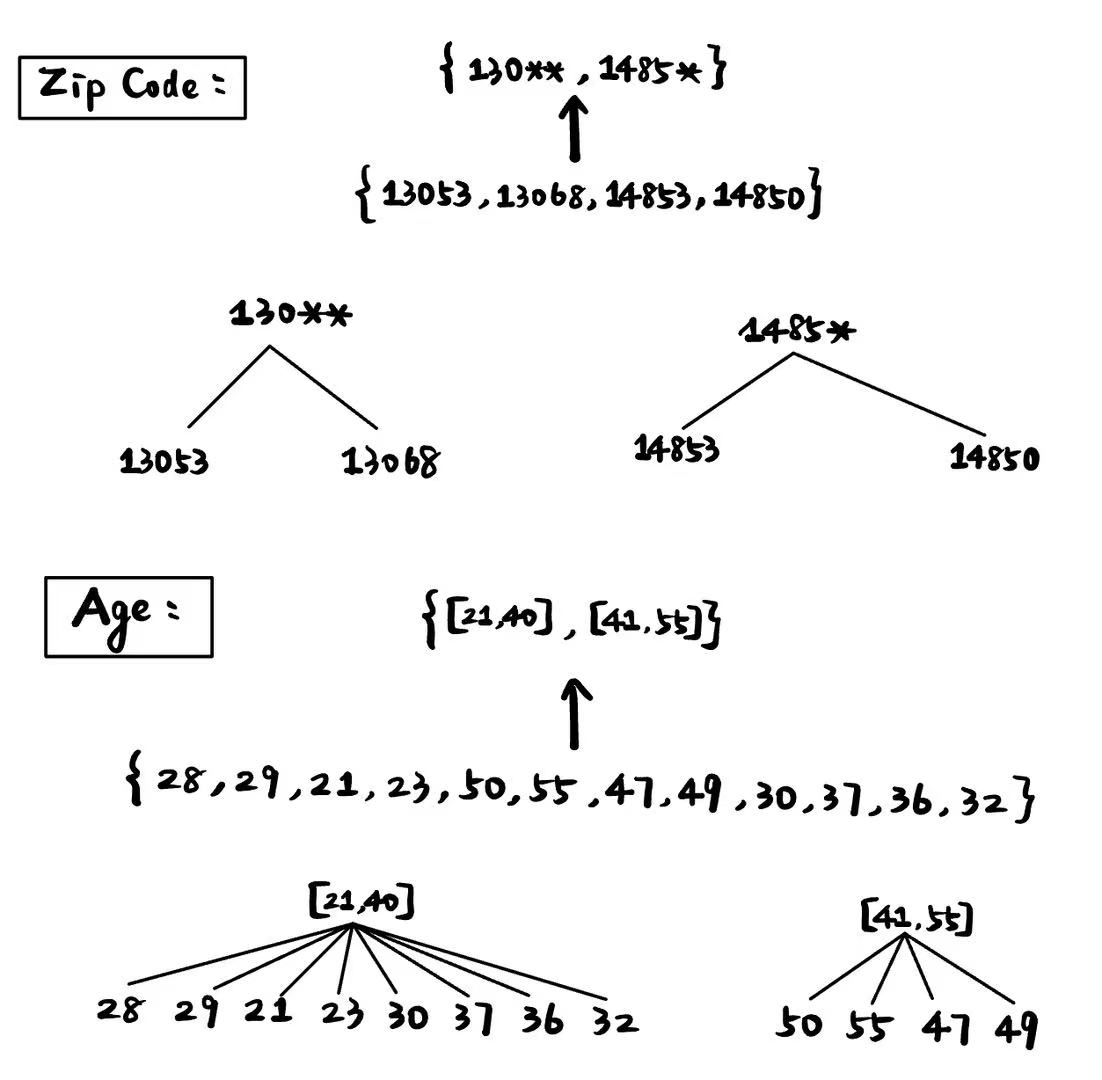
\includegraphics[width = 0.5\textwidth]{pics/pic1.jpg}
    \caption{generalization hierarchies}
    \label{fig:1}
\end{figure}
Figure \ref{fig:2}
\begin{figure}[htbp]
    \centering
    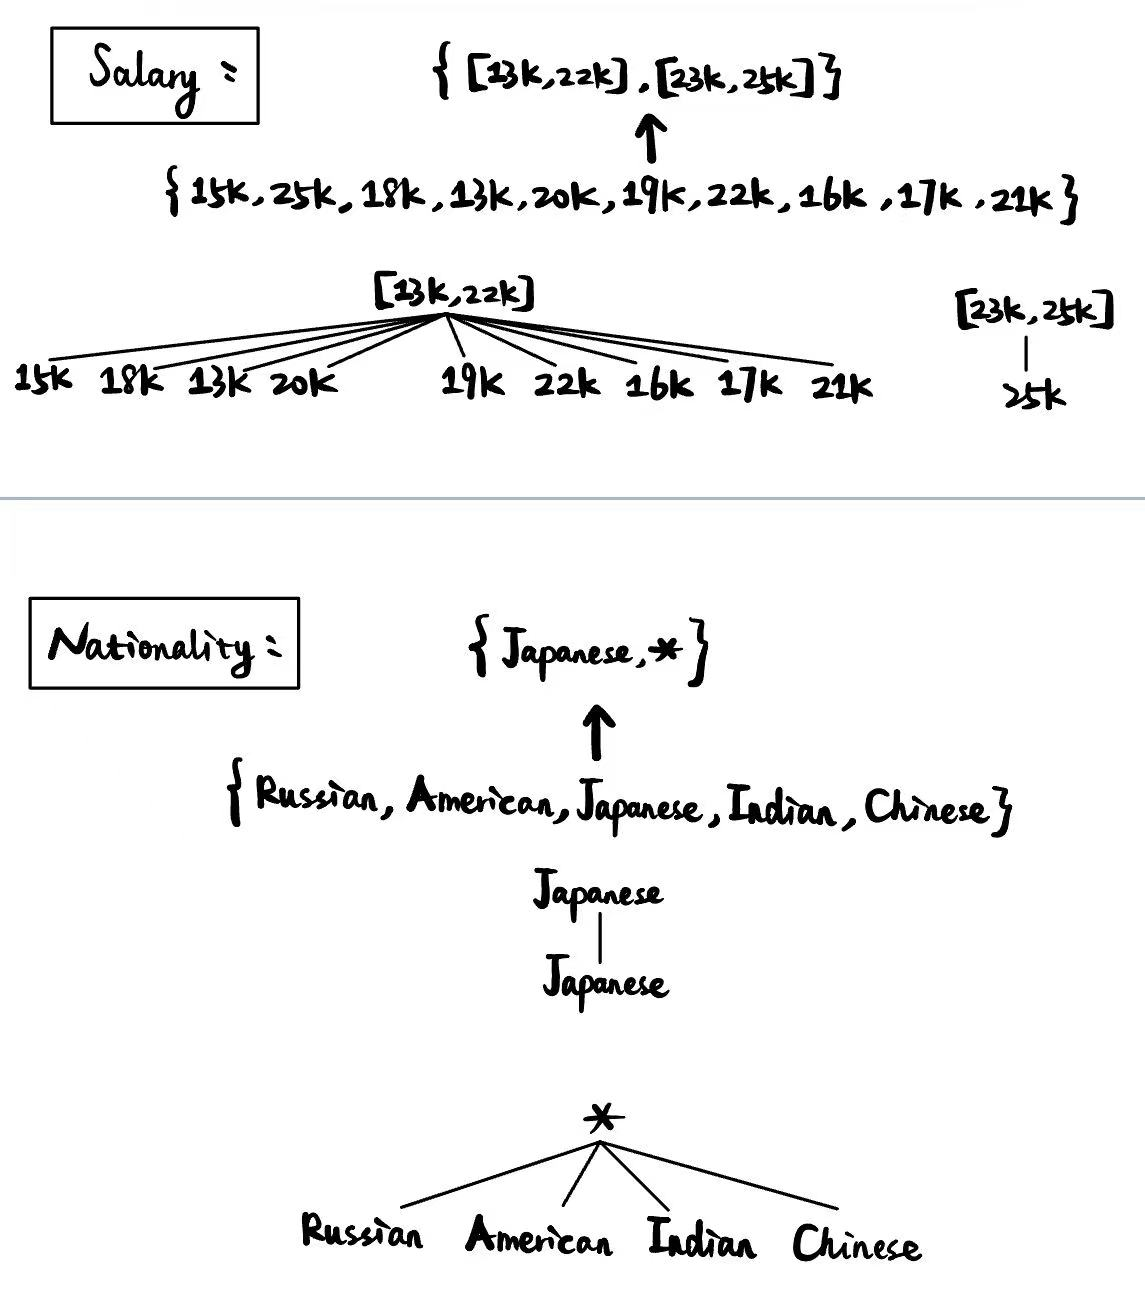
\includegraphics[width = 0.5\textwidth]{pics/pic2.jpg}
    \caption{generalization hierarchies}
    \label{fig:2}
\end{figure}
\newpage
Calculation of the LM:
\newline
\textbf{Zip Code:}
\newline
$T[13053]=\frac{2-1}{4-1}=\frac{1}{3}$
\newline
$T[13068]=\frac{2-1}{4-1}=\frac{1}{3}$
\newline
$T[14853]=\frac{2-1}{4-1}=\frac{1}{3}$
\newline
$T[14850]=\frac{2-1}{4-1}=\frac{1}{3}$
\newline
Therefore, $LM_{Zip Code}=\frac{1}{3}$
\newline
\textbf{Age:}
\newline
$T[21-40]=\frac{40-21}{55-21}=\frac{19}{34}$
\newline
$T[41-55]=\frac{55-41}{55-21}=\frac{14}{34}$
\newline
Therefore, $LM_{Age}=(8\times \frac{19}{34}+4\times \frac{14}{34})\times \frac{1}{12}=\frac{26}{51}$
\newline
\textbf{Salary:}
\newline
$T[13-22]=\frac{22-13}{25-13}=\frac{3}{4}$
\newline
$T[23-25]=\frac{25-23}{25-13}=\frac{1}{6}$
\newline
Therefore, $LM_{Salary}=(10\times \frac{3}{4}+2\times \frac{1}{6})\times \frac{1}{12}=\frac{47}{72}$
\newline
\textbf{Nationality:}
\newline
$LM_{Nationality}=\frac{3}{4}\times \frac{4}{5}=\frac{3}{5}$
\newline
In conclusion, $LM=\frac{1}{3}+\frac{26}{51}+\frac{47}{72}+\frac{3}{5}=\frac{12827}{6120}\approx2.1$

\section{Q2}
\subsection{a}
\textbf{meet recursive (2,2)-diversity}
\newline
Figure \ref{fig:5}
\begin{figure}[htbp]
    \centering
    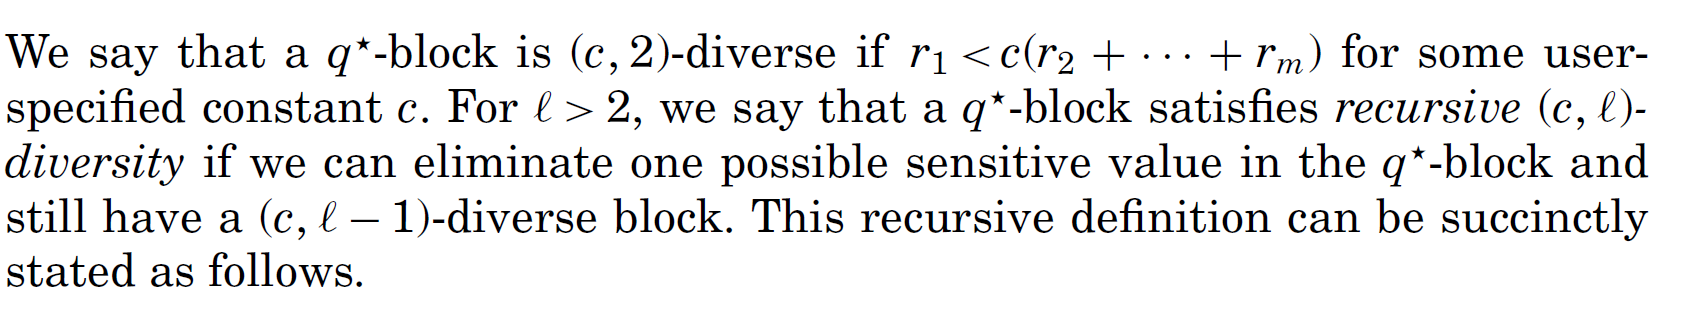
\includegraphics[width = 0.9\textwidth]{pics/pic5.png}
    \caption{recursive (c,l)-diversity definition}
    \label{fig:5}
\end{figure}
\newline
For every QI-cluster, we have $r_1=2,\ r_2=1,\ r_3=1$. So $r_1<2\times(r_2+r_3)$ holds (i.e. $2<2\times2$)
\subsection{b}
Entropy is a concave(the definition of \textbf{concave} may be vague) function. Thus if QI-cluster $q_1^\star,\ \cdots\cdots,\ q_d^\star$ from table T are merged
to form the QI-cluster $q^{\star\star}$ of table $T^{\star}$, then we have $entropy(q^{\star\star})\geq \min_i(entropy(q_i^\star))$
\newline
Since table T satisfies entropy l-diversity, we have $entropy(q^{\star\star})\geq \min_i(entropy(q_i^\star))\geq \log(l)$. Therefore, we get $T^\star$
satisfies entropy l-diversity.

\section{Q3}
\subsection{a}
To calculate EMD under ordered distance, we just need to consider flows that \textbf{transport distribution mass between adjacent elements}. This is
because other circumstances can be decomposed into several transportations between adjacent elements.
\newline
So let us consider element 1 first. Let us assume that $p_1-q_1<0$, so $q_1-p_1$ should be transported from other
elements to element 1.
\newline
We can transport this from element 2. So after transportation, element 2 has an extra amount of
$(p_1-q_1)+(p_2-q_2)$. The operation is similar element 3 $\cdots\cdots$
\newline
Therefore, we can get $D[\textbf{P,Q}]=\frac{1}{m-1}(|r_1|+|r_1+r_2|+\cdots+|r_1+r_2+\cdots+r_{m-1}|)$

\subsection{b}
$m=9,\ ordered\ list=\{3K,\ 4K,\ 5K,\ 6K,\ 7K,\ 8K,\ 9K,\ 10K,\ 11K\}$
\newline
Distribution of the whole table:
\newline
$\textbf{Q}=\{\frac{1}{9},\frac{1}{9},\frac{1}{9},\frac{1}{9},\frac{1}{9},\frac{1}{9},\frac{1}{9},\frac{1}{9},\frac{1}{9} \}$
\newline
Distribution of each cluster:
\newline
$\textbf{P}_1=\{0,\frac{1}{3},\frac{1}{3},\frac{1}{3},0,0,0,0,0\}$
\newline
$\textbf{P}_2=\{\frac{1}{3},0,0,0,0, \frac{1}{3},0,0,\frac{1}{3}\}$
\newline
$\textbf{P}_3=\{0,0,0,0,\frac{1}{3},0,\frac{1}{3},\frac{1}{3},0\}$
\newline
$D[\textbf{P$_1$,Q}]=\frac{1}{8}\times\frac{1}{9}(1+1+3+5+4+3+2+1)=\frac{5}{18}$
\newline
$D[\textbf{P$_2$,Q}]=\frac{1}{8}\times\frac{1}{9}(2+1+0+1+2+0+1+2)=\frac{1}{8}$
\newline
$D[\textbf{P$_3$,Q}]=\frac{1}{8}\times\frac{1}{9}(1+2+3+4+2+3+1+1)=\frac{17}{72}$
\newline
$t=\max\{D[\textbf{P$_1$,Q}],\ D[\textbf{P$_2$,Q}],\ D[\textbf{P$_3$,Q}]\}=\frac{5}{18}\approx0.278$

\section{Q4}
\subsection{a}
\textbf{question1:}
\newline
$P_{prior}(x=0)=0.01$
\newline
$P(R_1(x)=0)=0.3\times0.01+0.7\times\frac{1}{101}=0.00993$
\newline
$P_{posterior}(x=0|R_1(x)=0)=\frac{0.01\times(0.3+0.7\times\frac{1}{101})}{0.00993}=0.3091$
\newline
\textbf{question2:}
\newline
$P_{prior}=0.01$
\newline
$P(R_2(x)=0)=P(x+\xi=0)+P(x+\xi=101)=0.01\times\frac{1}{21}+10\times0.0099\times\frac{1}{21}+10\times0.0099\times\frac{1}{21}=0.00990$
\newline
$P(R_3(x)=0)=0.5\times0.00990+0.5\times\frac{1}{101}=0.00990$
\newline
$P_{posterior}(x=0|R_3(x)=0)=\frac{0.01\times(0.5\times\frac{1}{21}+0.5\times\frac{1}{101})}{0.00990}=0.0291$
\newline
\textbf{question3:}
\newline
$P_{prior}(x\in [20,80])=61\times0.0099=0.6039$
\newline
$P_{posterior}(x\in [20,80]|R_2(x)=0)=\frac{0}{0.00990}=0$
\subsection{b}
$R_3$ is more suitable. This is because $P_{posterior}$ should be close enough to $P_{prior}$, in this way we can protect the privacy.
Apparently, $R_3$ is closest to $nothing$ in both $X=0$ and $X\notin \{200, \cdots ,800\}$. Therefore, $R_3$ is more suitable.

\section{Q5}
\subsection{a}
Figure \ref{fig:3}
\begin{figure}[htbp]
    \centering
    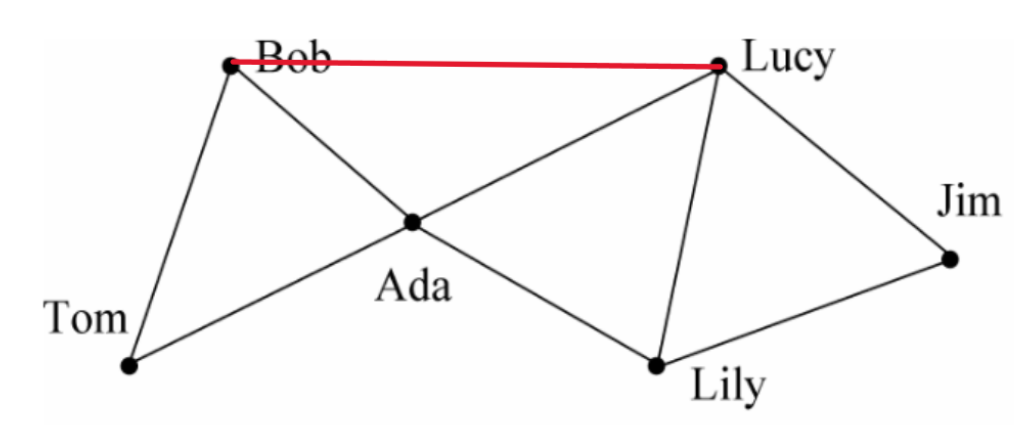
\includegraphics[width = 0.27\textwidth]{pics/pic3.png}
    \caption{2-anonymous}
    \label{fig:3}
\end{figure}
\subsection{b}
Figure \ref{fig:4}
\begin{figure}[htbp]
    \centering
    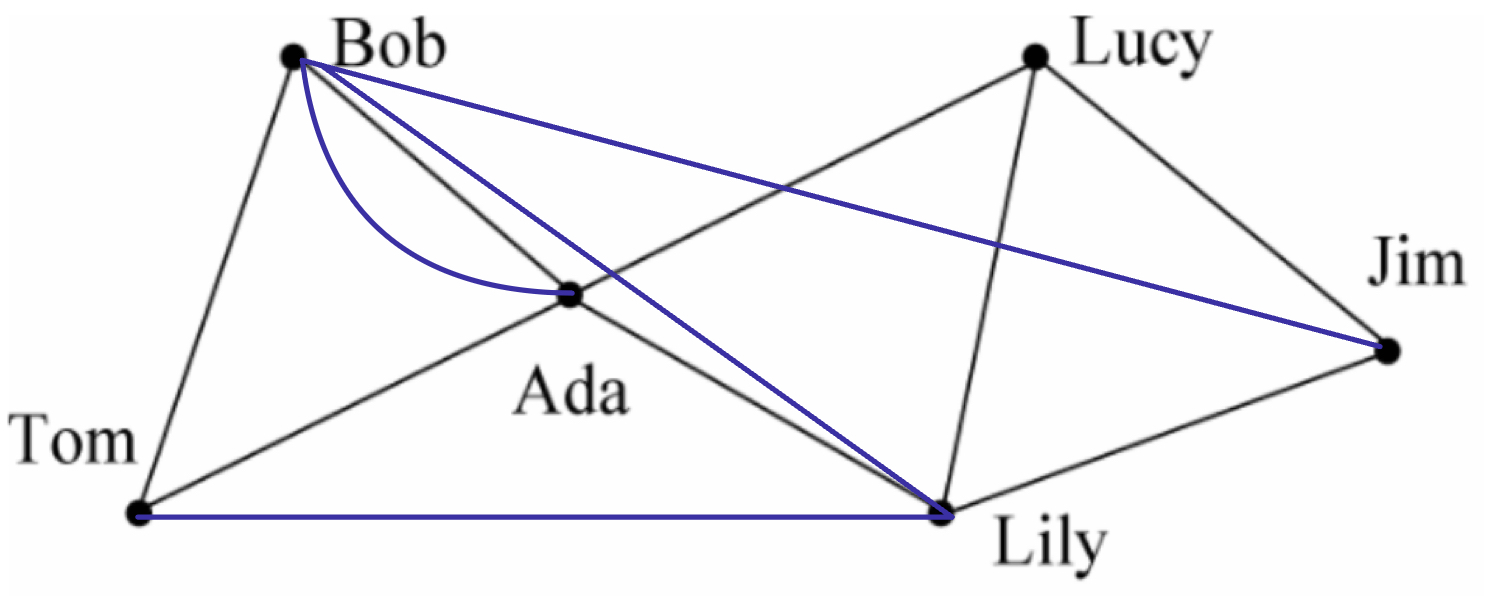
\includegraphics[width = 0.27\textwidth]{pics/pic4.PNG}
    \caption{3-anonymous}
    \label{fig:4}
\end{figure}
\subsection{c}
Figure \ref{fig:3}:
\newline
$L(G,G')=1-\frac{8}{9}=\frac{1}{9}$
\newline
Figure \ref{fig:4}:
\newline
$L(G,G')=1-\frac{8}{12}=\frac{1}{3}$

\end{document}